\chapter{IST-Analyse}
In dieser Arbeit wird man das Bestellsystem von der Party-Service-Website "Jungekueche". Dazu sind auch das Verwaltungssystem des Auftraggeber und die Verwaltungsseite des Kunden. Zuerst wird es User Interface von allen drei beschreiben, danach werden wir die Funktionalität dieses System betrachten.

\section{Beschreibung des User Interface (UI) des Bestellsystems} 

Die Anmeldung und die Registrierung Formular befindet sich auf einer gemeinsamen Seite. 
Die Anmeldung Formular hat zwei Felder, in denen den Benutzer seine PIN und E-Mail eingeben muss. Neben den Felder steht ein Hinweis, durch das den Kunde die nötige Information hat, wie sich anmelden oder sich registrieren kann.  


\begin{figure}[h]
	\centering
	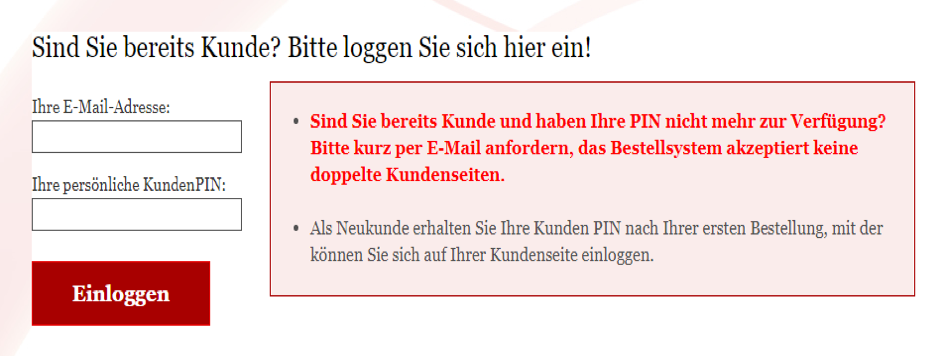
\includegraphics[width=0.7\linewidth]{/Users/matheo.zech/Documents/Thesis-Bozhidar/Graphics/anmeldeformular.png}
	\caption[Anmeldeformular]{Die bisherige Eingabemaske für den Kundenlogin}
	\label{fig:anmeldeformular}
\end{figure}


Falls den Kunde kein PIN hat, muss er sich registrieren. Dies Formular besteht auf fünf Sektionen. Im ersten muss der Kunde seine persönlichen Daten geben. In der zweiten stehen die Angeben zum Auftrag. Menü Auswahl it die nächste Sektion. Im vorletzten stehen die Zubehörauswahl und Serviceauswahl. Das letzte Sektion ist die Erklärungen zu dem Registrierungsprozess. 

\begin{figure}
	\centering
	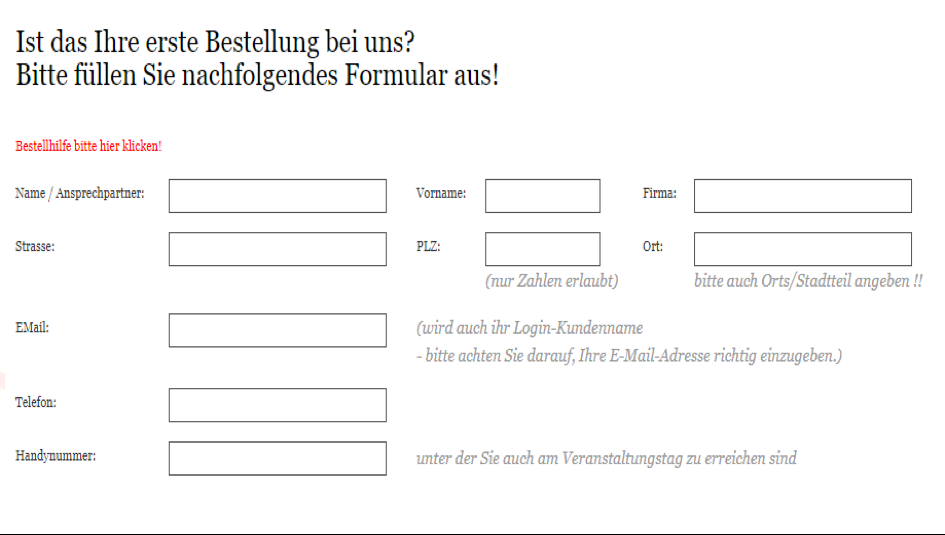
\includegraphics[width=0.7\linewidth]{/Users/matheo.zech/Documents/Thesis-Bozhidar/Graphics/registerForm.png}
	\caption[Registerformular]{Die bisherige Eingabemaske für den Registerformular}
	\label{fig:registerForm}
\end{figure}

Bei einer Registrierungsanftage kann der Auftraggeber sie bestätigen oder löschen. Für besseres Verständnis, was der Auftraggeber machen kann, werden wir uns mit der Verwaltungsseite des Auftraggeber. Sie besteht auf drei Optionen: Auftragsverwaltung, E-Mail Verwaltung und Umsatzverwaltung. Zuerst werden wir die Auftragsverwaltung betrachten. Da befindet sich elf Optionen, neun davon zum eigene Unteroptionen weiteleiten. Andere zwei sind "Save" und "Abmelden". Durch diese Optionen kann der Auftraggeber die Kunde einsehen, editieren, kommunizieren und löschen, dazu die Nachrichten einlesen oder löschen. Er kann nicht nur das machen, sonder auch die neuen/bearbeitenden/alten Aufträge einsehen, editieren oder löschen.

\begin{figure}[h]
	\centering
	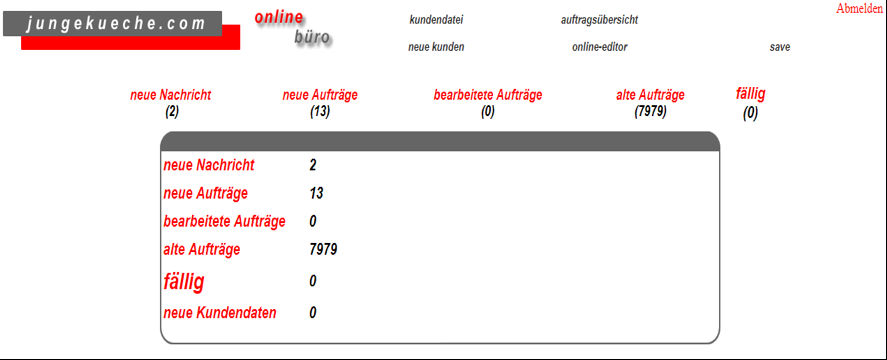
\includegraphics[width=0.7\linewidth]{/Users/matheo.zech/Documents/Thesis-Bozhidar/Graphics/Auftragverwaltung.png}
	\caption[Auftragsverwaltung]{Die bisherige Eingabemaske für den Auftragsverwaltung}
	\label{fig:Auftragverwaltung}
\end{figure}

Wenn die Anfrage des Kunden bestätigt wird, bekommt der Kunde ein PIN pe E-Mail. Mit diesem PIN und seinem E-Mail kann der Kunde sich im "Jungekueche" anmelden. Danach er wird in seiner persönlichen Seite eingelogt. Dort hat er eine Übersicht auf seine aktuelle und alte Bestellungen, ein Kontaktfenster, in dem er die Nachrichten einsehen oder neue schreiben kann, Wichtige Information und Information zu Beachten. Es gibt eine Option, durch die den Kunde neue Bestellungen machen kann.  

\begin{figure}[h]
	\centering
	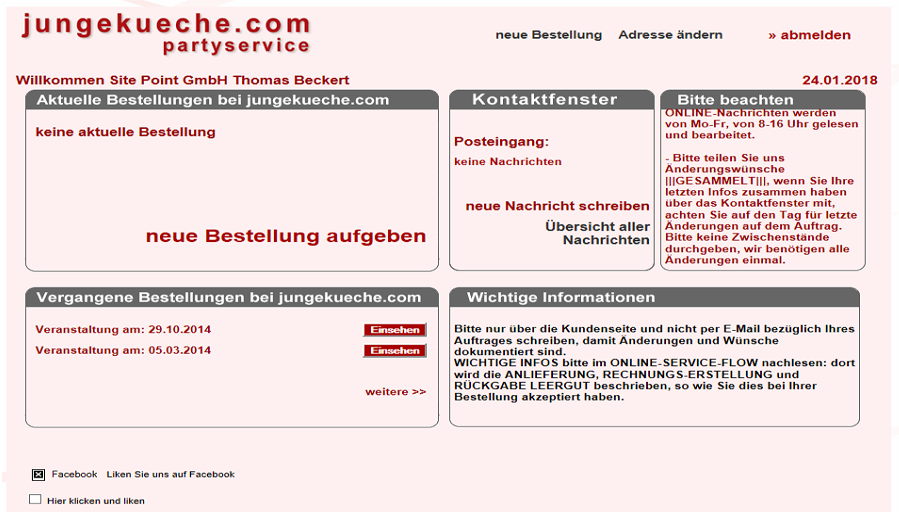
\includegraphics[width=0.7\linewidth]{/Users/matheo.zech/Documents/Thesis-Bozhidar/Graphics/KundenAnsicht.png}
	\caption[Kundeansicht]{Die bisherige Eingabemaske für den Auftragsverwaltung}
	\label{fig:KundenAnsicht}
\end{figure}

\section{Beschreibung der Funktionalität}   

Man hat schon erfahren, dass die Anmeldung ist von dem Registrierung abhängig. Jetzt wird es erläutert. Das Programm wie schon besagt wurde, ist auf ASP und ASP.NET basiert. Die verwendenden Hilfsprogrammen sind JQuery, JavaScript, AJAX, HTML und CSS. 

Zuerst wird es betrachtet, wie funktioniert die Kommunikation zwischen den Datei. Das ganze Programm besteht aus Fron- und Backend. Frontend ist diese Teil, die der Benutzter verwendet. Im Backend werden die Daten verarbeitet. Die Verbindung zwischen die beiden ist wegen JavaScript und JQuery  Methoden. Wenn der Benutzer eine Tätigkeit tätigen, werden die eingegebenen Eingaben über JavaScript Methoden zu dem Backend weitergeleitet. Dort werden sie verarbeitet und werden über JavaScript Methode aufgerufen, und werden wieder zu dem Frontend zugeschickt. Das Backend entsteht aus ASP-Datei, in denen sich verschiedenen Methoden befindet, und Datenbanken. In der Datenbanken werden die eingegebenen Eingaben gespeichert.    




Abbildung (neue Diagramm.. die Kommunikation zwischen Front- und Backend bzw. Client -Server)

Jetzt, wenn man verstanden hat, wie funktioniert die Kommunikation zwischen Front- und Backend, soll man verstehen, wie die verschiedene Befehle vom Frontend zu dem Backend passieren. 

\subsection{Anmelde- und Registerformular} 

Es wird mit dem Bestellseite angefangen, bzw. Anmeldeformular. Wenn die Kunde "Anmeldung" drückt, wird eine HTML Post-Methode aktiviert.  So werden JavaScript- und ASP- Methoden aufgerufen. Die JavaScript-Methoden werden benutzt, damit die Eingabe geprüft wird, ob sie korrekt ist, und ASP-Methoden werden dann aufgerufen. 

Der Registerformular funktioniert auf demselben Prinzip. Wenn die Eingaben eingegeben sind, werden sie geprüft, ob alles korrekt ist, falls alles in Ordnung ist, werden die Eingaben zu dem zugeordneten Daten, bzw. Methoden zugeschickt.

mehr im Anhang - Funktionen

\begin{figure}[h]
	\centering
	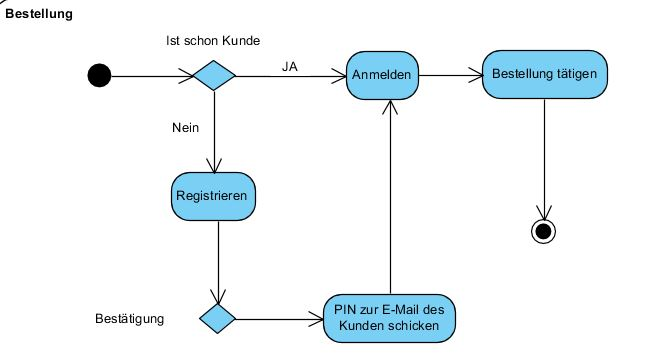
\includegraphics[width=0.9\linewidth]{/Users/matheo.zech/Documents/Thesis-Bozhidar/Graphics/Bestellung.JPG}
	\caption[Anmeldung/Bestellung]{Die bisherige Eingabemaske für den Vorgang der Bestellung/Registrierung}
	\label{fig:Bestellung}
\end{figure}

\subsection{Auftraggeber-Verwaltung}

Hier wird man sich nur mit dem Auftragsverwaltung beschäftigen. Die Auftragsverwaltung, wie es schon beschrieben wurde, besteht auf verschiedenen Optionen. Jetzt lässt sich jeweiliges betrachten, wie es funktioniert. 
	
\subsubsection{Nachricht-Sektion} ermöglicht dem Auftraggeber die Information zu lesen oder löschen. Nach zugeordnetem Wahl wird die Information in der Datenbank "komentar" entweder aufgerufen oder entfernt. 

\begin{figure}[h]
	\centering
	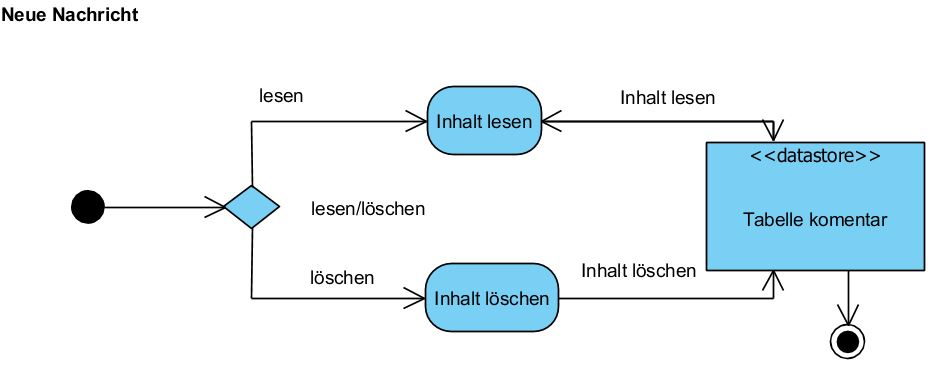
\includegraphics[width=0.8\linewidth]{/Users/matheo.zech/Documents/Thesis-Bozhidar/Graphics/NeueNachricht.JPG}
	\caption[Kommunikation]{Die bisherige Eingabemaske für den Nachrichten lesen oder löschen}
	\label{fig:Kommunikation}
\end{figure}



\subsubsection{Aufträge: Neue, alte und bearbeitende}

Die Funktionalität von allen drei ist dieselbe. Deswegen es wird allgemein erklärt. Der Auftraggeber kann den Auftrag sehen, editieren oder löschen. Alle von diese Aktivitäten ist mit mehrere Datenbanken verbunden, die verschiedenen Informationen über die gewählten Artikel haben. In den Abbildungen \ref{fig:Autrag_Loeschen} und \ref{fig:auftragEinsehen} betrachtet man die jeweilige Funktionalität.


\begin{figure}[h]
	\centering
	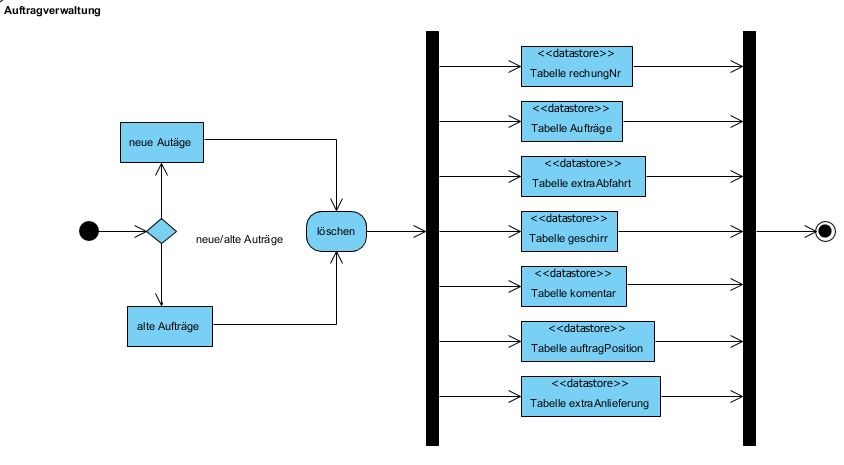
\includegraphics[width=1\linewidth]{/Users/matheo.zech/Documents/Thesis-Bozhidar/Graphics/Autrag_Loeschen.JPG}
	\caption[AutragLoeschen]{Die bisherige Eingabemaske für den Nachrichten lesen oder löschen}
	\label{fig:Autrag_Loeschen}
\end{figure}
 
\begin{figure}[h] 
	\centering
	\includegraphics[width=1\linewidth]{/Users/matheo.zech/Documents/Thesis-Bozhidar/Graphics/auftragVerwaltung.JPG}
	\caption[auftragEinsehen]{Die bisherige Eingabemaske für den Nachrichten lesen oder löschen}
	\label{fig:auftragEinsehen}
\end{figure}

\pagebreak
\subsubsection{Kundendatei}

Hier befindet sich die Information über die Kunden. Da kann man die Information editieren oder löschen. Um der bestimmten Kunde schneller zu finden, steht eine Suchmaschine zur Verfügung. Eine bessere Übersicht stellt uns die Abbildung dar. 

Abbildung Adressbuch

Wenn man editieren oder löschen will, wird es über JavaScript Funktion passiert. Diese Funktion ruft die Methoden auf, die sich in der zugeordneten ASP-Datei befindet. Im "Editor-Fenster" kann man die Daten des Kunden editieren, Login-Daten wie Email an Kunden übermitteln, Wichtige Information für alle Kunden senden, V.I.P-Status des Kunden geben, spezifische Warnungen jeweiligem Kunde aufgeben, Information schreiben, sowie Unterschrift editieren und etc. Besser Verständnis zum diesen Fenster ergibt uns Abbildung 3-19

Abbildung übersicht von Editor-Fenster

Durch JavaScript - Methode wird eine zusätzlichen Möglichkeit zu dem Kunde Nachricht geschrieben zu werden. Sie wird aktiviert, wenn der Cursor auf dem bestimmten Kunde, der in der Liste des Adressbuch ist, steht. Die Kommunikation zwischen dem Auftraggeber und dem  Kunde wird auch im Datenbank "komentar" gespeichert. 

Abbildung Neue Nachricht

Nach allem, was geschrieben ist, soll man sich ein vertieftes Verständnis aufbauen. In folgender Abbildung kann man wie genau die Aktivitäten des Auftraggeber passieren und wie funktioniert die Nachricht-Kommunikation.

Abbildung Kundendatei

Abbildung Auftraggeber-Kunde  

\subsubsection{Online-Editor}

Durch diese Option kann man die neuen Artikel zu erstellt, editieren und löschen werden können.  Es gibt „Artikel – Arragements“ und „Artikel – Standard“. Wenn schon ein Artikel erstellt wurde, kann er entweder gelöscht, editiert oder zugeordnet werden. 
JavaScript Funktionen werden benutzt, um die Eingabe zu prüfen, ob alles korrekt ist. Wenn alles in Ordnung ist, werden die obengenannten Methoden aus den jeweiligen Dateien aufgerufen. In der folgenden Abbildung ist die Übersicht der Sete zu sehen.

Abbildung Online Übersicht

Wenn die Option „Editieren“ zu dem „Artikel-Arrangements“ ausgewählt wird, wird neue Seite geöffnet, in der es vielfältige Möglichkeiten gibt, die Inhalt geändert werden kann. Abbildung   zeigt uns wie diese Seite aussieht.

Abbildung

Artikel-Standard“ hat nur eine Möglichkeit, editiert zu werden. Sie wird in der Abbildung   dargestellt.


In der folgenden Abbildung ist der Zusammenhang zwischen die verschiedenen Funktionen des „Online-Editor“ zu sehen.

Abbildung Online-Editor



\section{Testen} 


Für diese Arbeit wird ein webbasierten Sicherheit-Checker von 1\&1. Nach eine vertiefte Recherche, zeigte sich, dass die Webseite auf eine mittlere Sicherheitsposition steht. Die Webseite ist nach vier Kriterien ohne Beanstandung abgesichert.

\begin{itemize}	
	
\item Secure Sockets Layer (SSL) Verschlüsselung – Über SSL wird sichergestellt, dass zwischen User und Server die übertragenen Daten nicht gelesen werden können.

\item Cookies sind auch sicher und so ist der Browser von Dritten über JavaScript unlesbar.

\item Apache-Status ist verboten. Die Status-Seite ist öffentlich nicht erreichbar. So wird den Schutz von potenziellen Angreifern erhöht. 

\item Server Version ist nicht sichtbar. Die Server Version ist öffentlich nicht einsehbar. Damit kann ein Angreifer nicht einfach bekannte Schwachstellen ausnutzen.

\end{itemize}

